\begin{frame}[plain,label=u1_title]{}
\titlepage
\end{frame}

\begin{frame}[label=u1_selection]{Training selection: PbPb 2023}
\begin{columns}[T]
\column{0.46\textwidth}\small
\textbf{Common selection: MC and DATA}
\begin{center}
\begin{tabular}{@{}ll@{}}\toprule
Variable & Selection before ML\\\midrule
\var{Bpt} & $15 < \var{Bpt} < 50$ GeV\\
\var{By} & $|\var{By}| < 1.6$\\
\var{BQvalue} & $\var{BQvalue} < 0.15$ GeV\\
\var{Btrk2dR} & $\var{Btrk2dR} < 0.35$\\\bottomrule
\end{tabular}\end{center}
\column{0.50\textwidth}\small
\textbf{Signal: X MC}\par
All pthat components; \var{pThatreweight}.\par
No additional mass window in training.\par\medskip
\textbf{Background: DATA sidebands}\par
$3.80 < m < 3.85$ or $3.89 < m < 3.94$ GeV.\par
Unit event weights.\par\medskip
\end{columns}
\end{frame}

\begin{frame}[label=u1_variables]{Variable selection from two to nine inputs}
\begin{columns}[T]
\column{0.51\textwidth}\small
\textbf{Allowed pool: 19 inputs}\par\medskip
\var{Btrk1dR}, \var{Btrk2dR}\par
\var{Btrk1Pt}, \var{Btrk2Pt}, \var{BtrkPtimb}\par
\var{Bmu1pt}, \var{Bmu2pt}\par
\var{Bmu1eta}, \var{Bmu2eta}\par
\var{Btrk1Eta}, \var{Btrk2Eta}\par
\var{Bujeta}, \var{Btktkpt}, \var{Btktketa}\par
\var{Bchi2Prob}, \var{BujvProb}, \var{BtktkvProb}\par
\var{Balpha}, \var{Bcos_dtheta}\par\medskip
\column{0.45\textwidth}\small
\begin{block}{Start point: two variables}
\var{Btrk1dR} + \var{Btrk2Pt}
\end{block}
\medskip
\textbf{Add according to AUC}\par
Evaluate additions from the allowed pool.\par
Rank by pooled train + test AUC.\par
Select the next variable combination.\par
\end{columns}
\end{frame}

\begin{frame}[label=u1_auc]{AUC: the new two- to nine-variable route}
\begin{columns}[T]
\column{0.68\textwidth}\centering
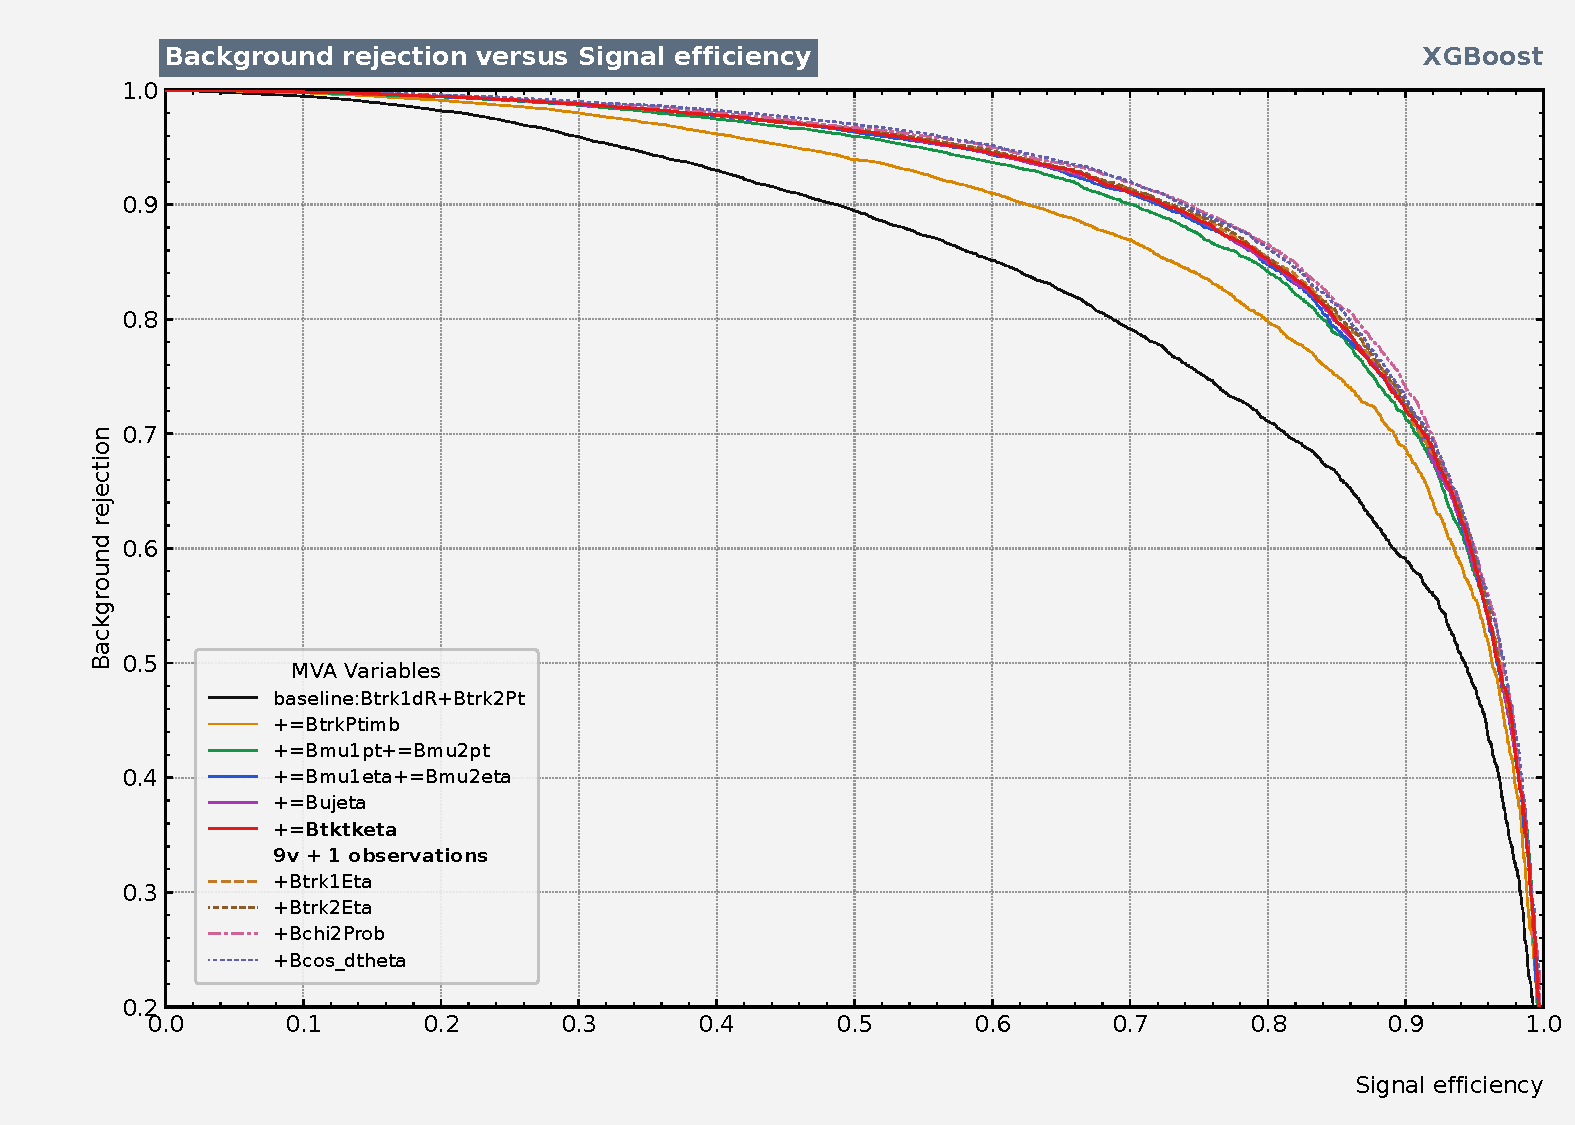
\includegraphics[width=\linewidth,height=0.73\textheight,keepaspectratio]{figures/20260924/auc.pdf}
\column{0.29\textwidth}\small
\textbf{Start point}\par
\var{Btrk1dR}\par
\var{Btrk2Pt}\par\medskip
\textbf{Endpoint: selected variables}\par
\var{Btrk1dR}, \var{Btrk2Pt}\par
\var{BtrkPtimb}\par
\var{Bmu1pt}, \var{Bmu2pt}\par
\var{Bmu1eta}, \var{Bmu2eta}\par
\var{Bujeta}, \var{Btktketa}
\end{columns}
\end{frame}

\begin{frame}[label=u1_formula]{Punzi FOM: empirical corrected form}
\small
Signal: $(3.84,3.90)$ GeV; sidebands: $(3.75,3.84)\cup(3.90,3.99)$ GeV.\par
\[
\mathrm{FOM}_{\rm corr}(c)=
\frac{\epsilon_X(c)}{\displaystyle
 a^2/8+9b^2/13+a\sqrt{B(c)}+
 \frac{b}{2}\sqrt{b^2+4a\sqrt{B(c)}+4B(c)}} ,\quad a=b=5.
\]
\begin{itemize}
\item $B(c)$: DATA sideband count after the score cut, divided by 3.
\item $\epsilon_X(c)$: weighted X MC efficiency for score $>c$, within $3.62<m<4.00$ GeV.
\item MC weight: \var{pThatreweight}; MC window factor fixed to 1.
\item $a$: discovery threshold; $b$: target power parameter.
\end{itemize}
\end{frame}

\begin{frame}[label=u1_punzi]{Nine-variable model: Punzi FOM versus score}
\begin{columns}[T]
\column{0.68\textwidth}\centering
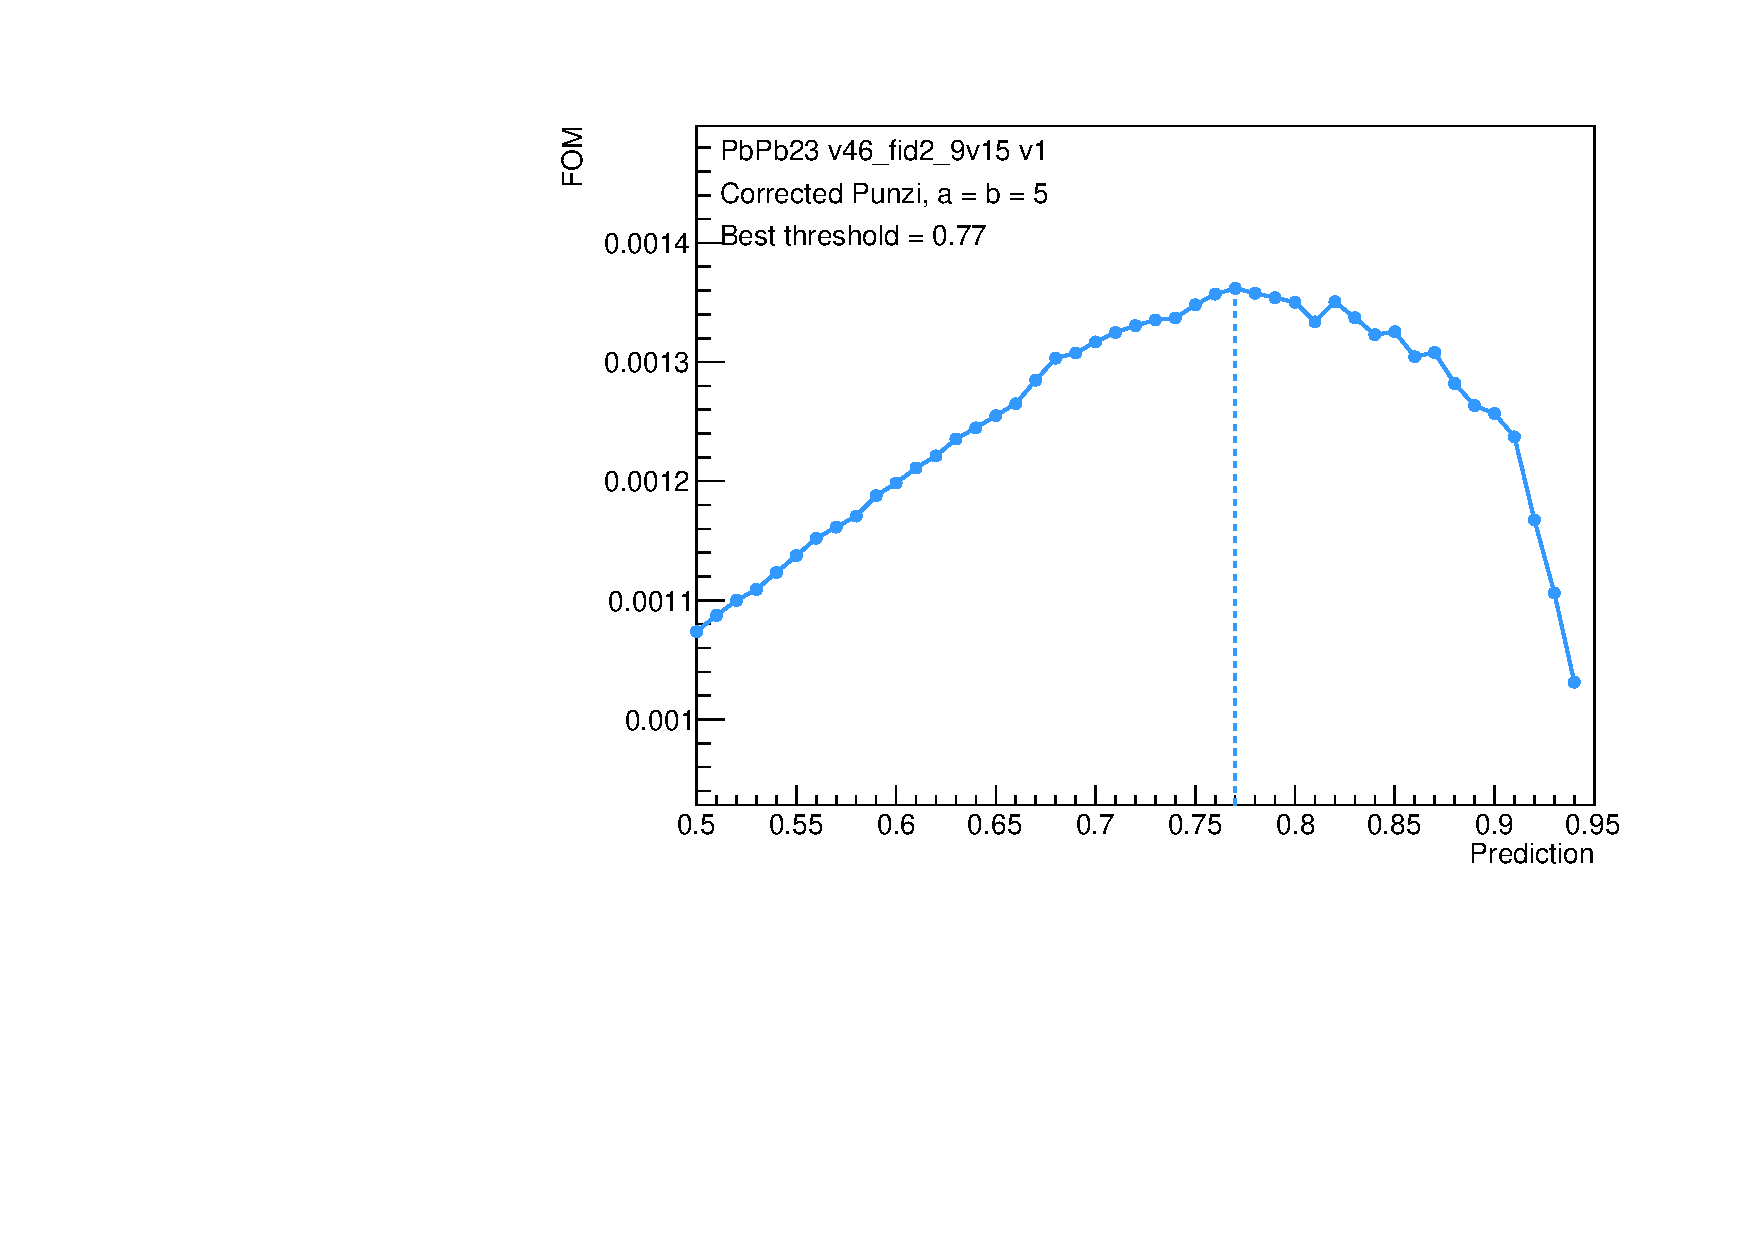
\includegraphics[width=\linewidth,height=0.73\textheight,keepaspectratio]{figures/20260924/main_9v_punzi_score.pdf}
\column{0.29\textwidth}\small
\textbf{Empirical corrected Punzi}\par
$a=b=5$.\par\medskip
Score: 0.50--0.95\par
Step: 0.01\par\medskip
\textbf{Grid maximum}\par
score $>0.77$\par
FOM $=1.361820\times10^{-3}$\par\medskip
\end{columns}
\end{frame}

\begin{frame}[label=u1_fit]{Nine-variable model: two-peak fit at the Punzi optimum}
\begin{columns}[T]
\column{0.65\textwidth}\centering
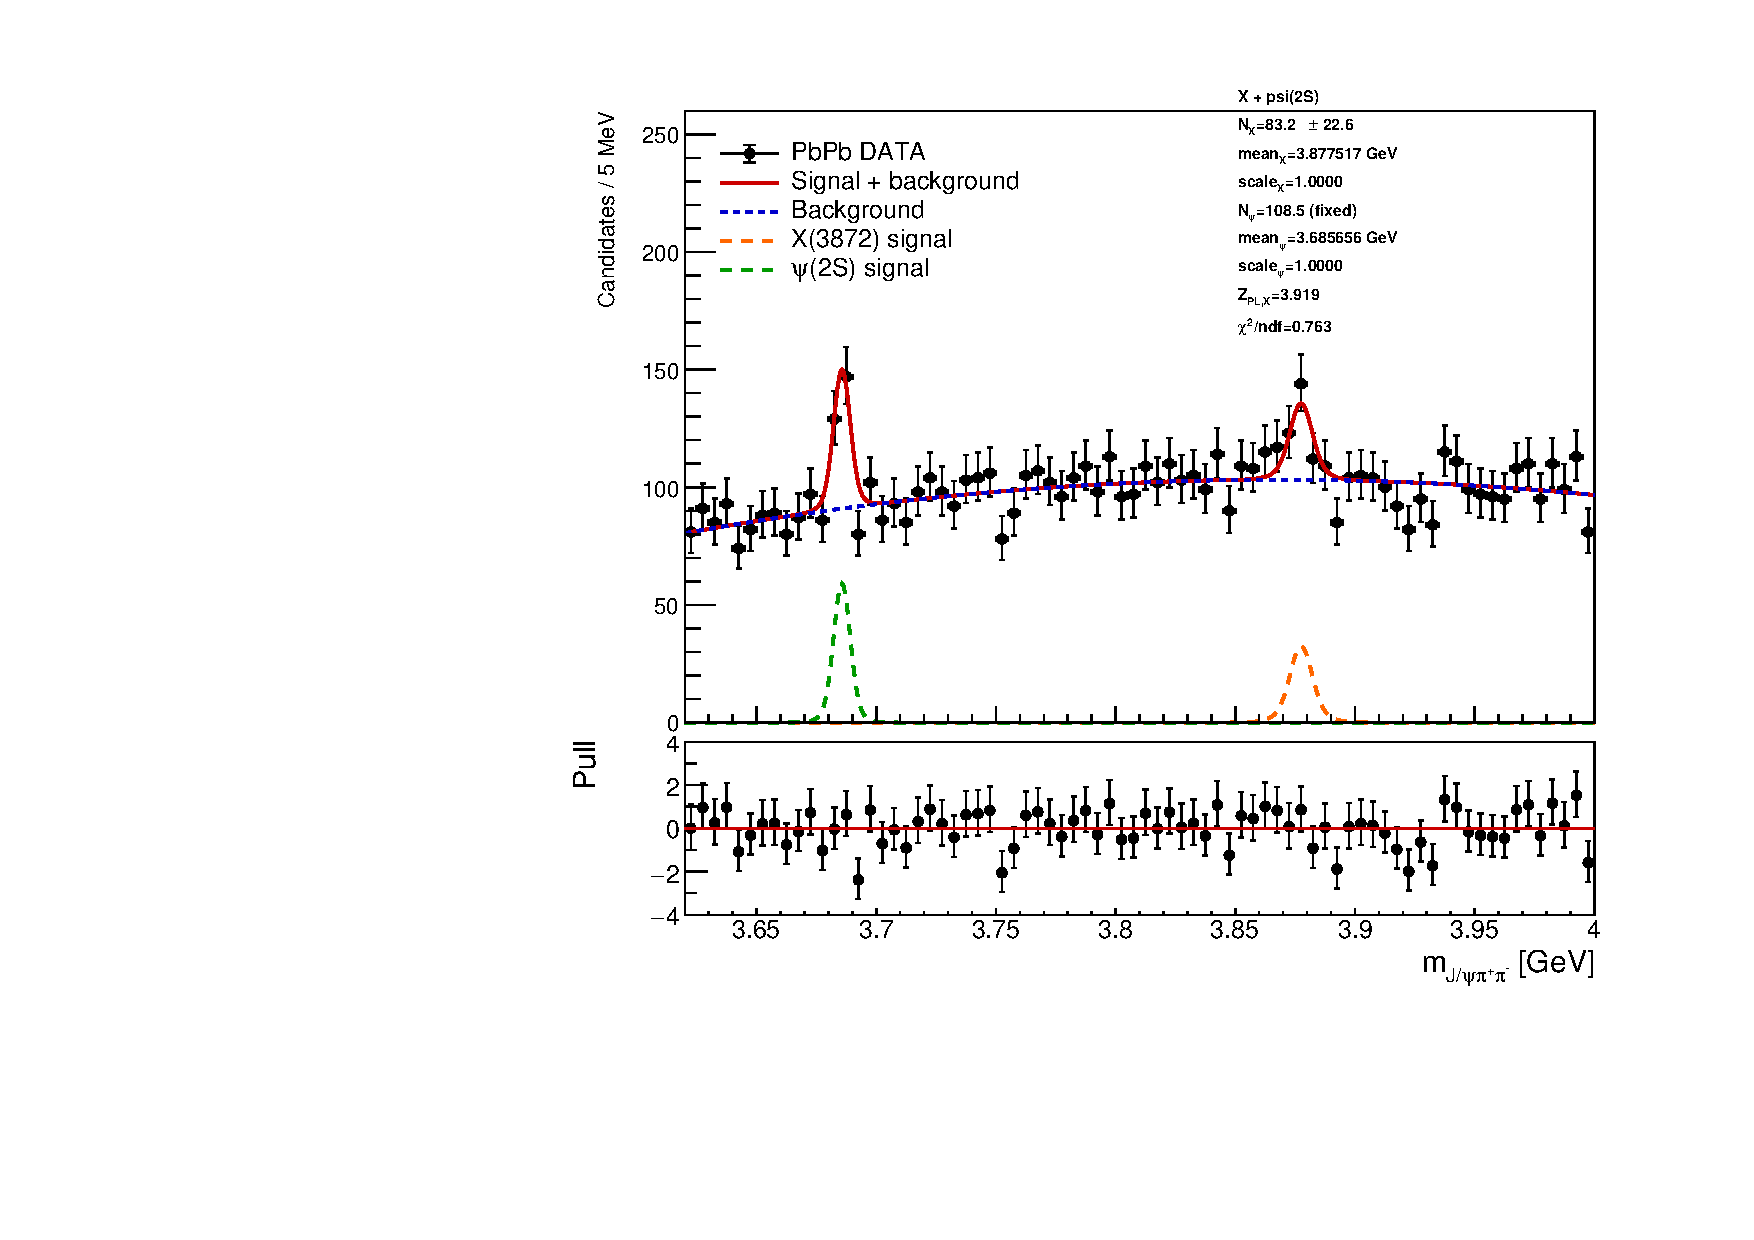
\includegraphics[width=\linewidth,height=0.72\textheight,keepaspectratio]{figures/20260924/main_9v_conditional_fit.pdf}
\column{0.32\textwidth}\small
\textbf{score $>0.77$}\par\medskip
$N_X=83.20\pm22.64$\par
$N_{\psi(2S)}=108.53$ (fixed)\par\medskip
$\sqrt{q_0}=3.919$\par\medskip
MC double-Gaussian widths fixed.\par
2nd-order Chebyshev background.
\end{columns}
\end{frame}

